%================================================================
\section{Results and Discussion}\label{sec:Results}
%================================================================

%===============================================================
\subsection{Heat Equation}\label{sec:heateq results}
%===============================================================
Accompanying notebook: \href{https://github.com/nicolossus/FYS-STK4155-Project3/blob/master/notebooks/heat_pde_with_fe_and_tf.ipynb}{heat\_pde\_with\_fe\_and\_tf.ipynb}.

%===============================================================
\subsubsection{Forward Euler}
%===============================================================
Nx = 11
Nt = 199

Max diff: 0.04009472326320718
Mean diff: 0.003186288853514369

\autoref{fig:heat_fe}
\begin{figure}[H]
\centering
\subfloat[]{{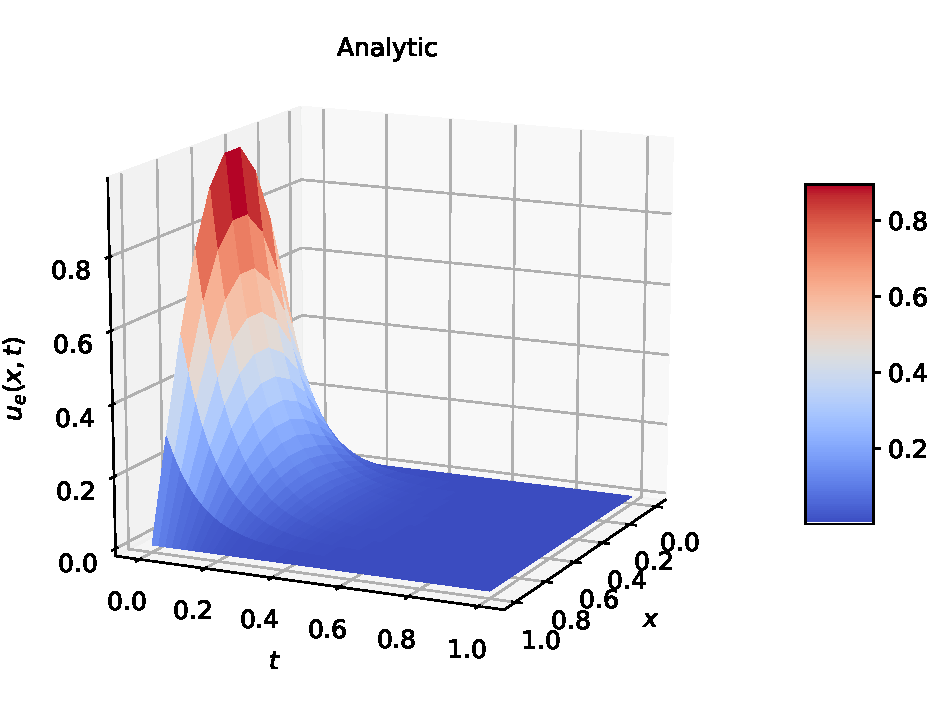
\includegraphics[scale=0.48]{latex/figures/heat_ana_fe.pdf}}}
\qquad
\subfloat[]{{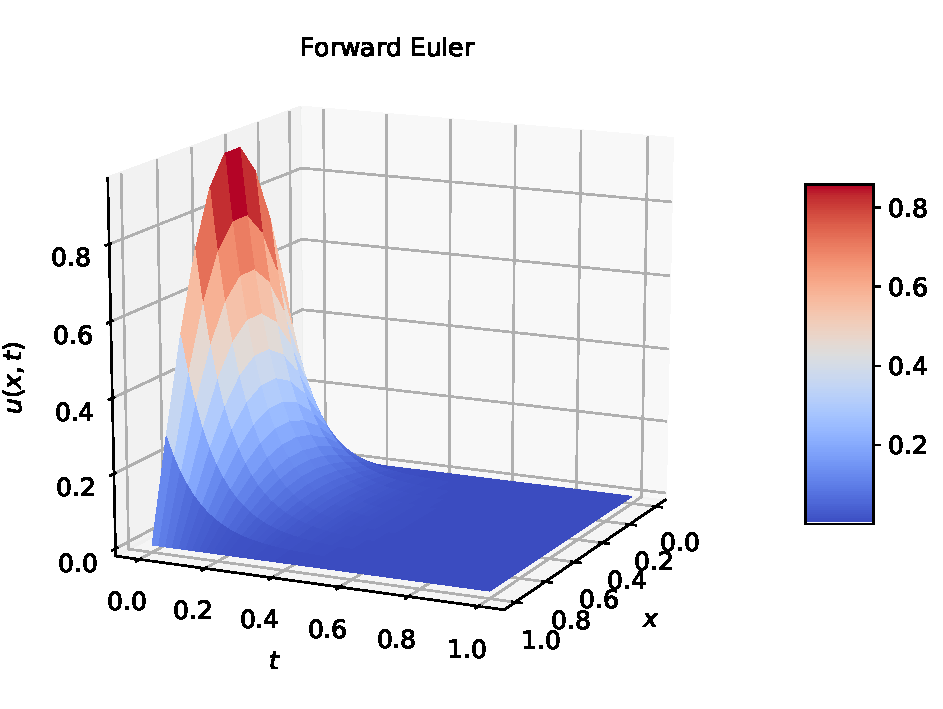
\includegraphics[scale=0.48]{latex/figures/heat_fe.pdf}}}
\qquad
\subfloat[]{{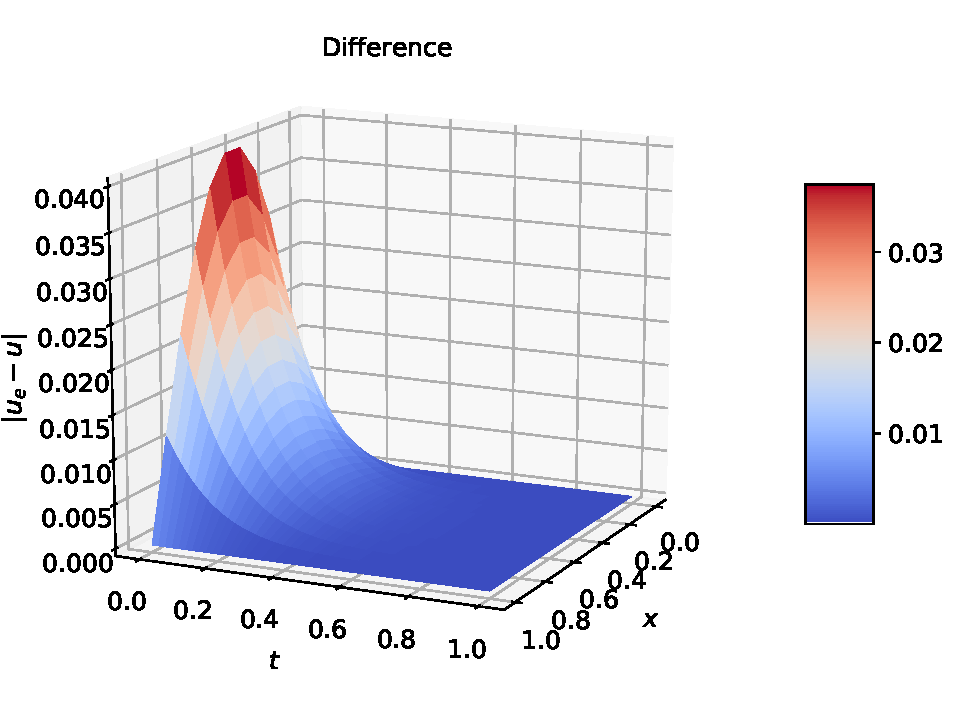
\includegraphics[scale=0.5]{latex/figures/heat_diff_fe.pdf}}}
\caption{FE heat}
\label{fig:heat_fe}
\end{figure}

CPU benchmark
Number of iterations: 1000
FE mean CPU time: 0.00158 secs

Simulations with the Forward Euler scheme show that the time step restriction, $F \leq 1/2$, which means $\Delta t \leq \Delta x^2 / (2\alpha)$, may be relevant in the beginning of the diffusion process, when the solution changes quite fast, but as time increases, the process slows down, and a small $\Delta t$ may be inconvenient.

%===============================================================
\subsubsection{FFNN Model 1}
%===============================================================

Model 1: Train on spatial and temporal points as dictated by FE stability criterion

Nx = 11
Nt = 199
2 layers + output, [150, 50, 1], [tanh, sigmoid, none] 
1000 epochs
Adam, initial lr=0.01
Step: 1000, Loss: 0.008064055285575904
Training FFNN CPU time: 147.62562 secs

\autoref{fig:heat_nn1} Plot solution on the grid FFNN is trained on

Max diff: 0.008466789818225778
Mean diff: 0.0029635112954797672

\begin{figure}[H]
\centering
\subfloat[]{{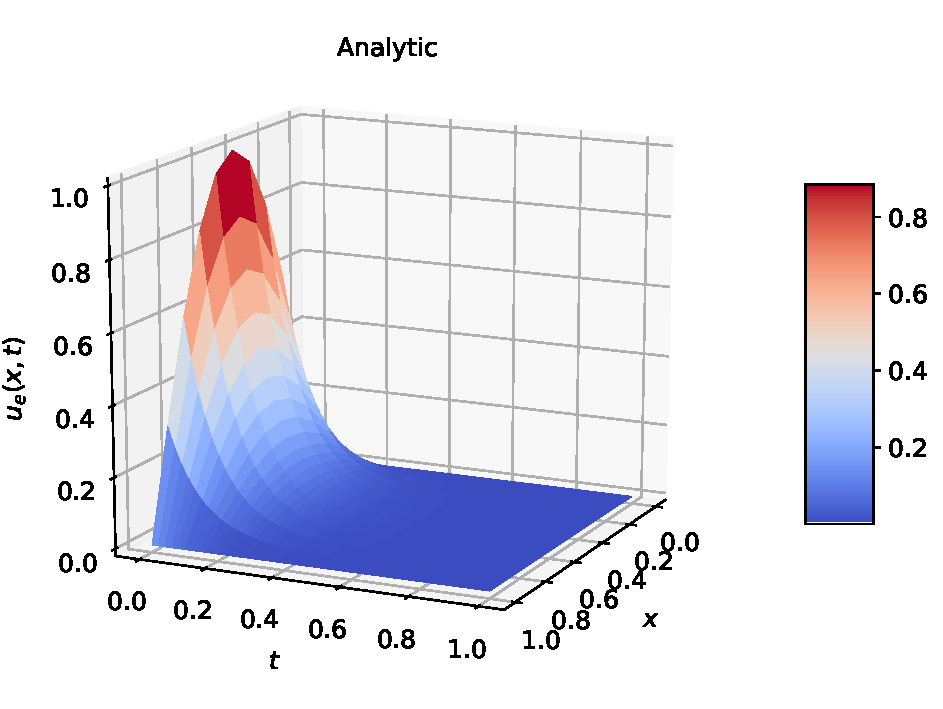
\includegraphics[scale=0.48]{latex/figures/heat_ana_nn1.pdf}}}
\qquad
\subfloat[]{{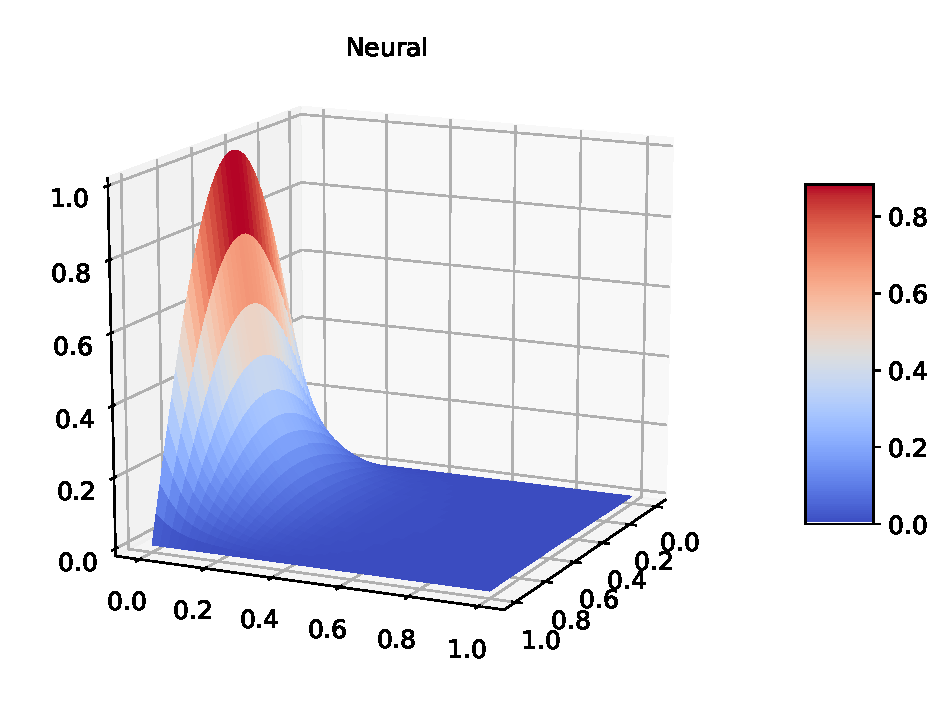
\includegraphics[scale=0.48]{latex/figures/heat_nn1.pdf}}}
\qquad
\subfloat[]{{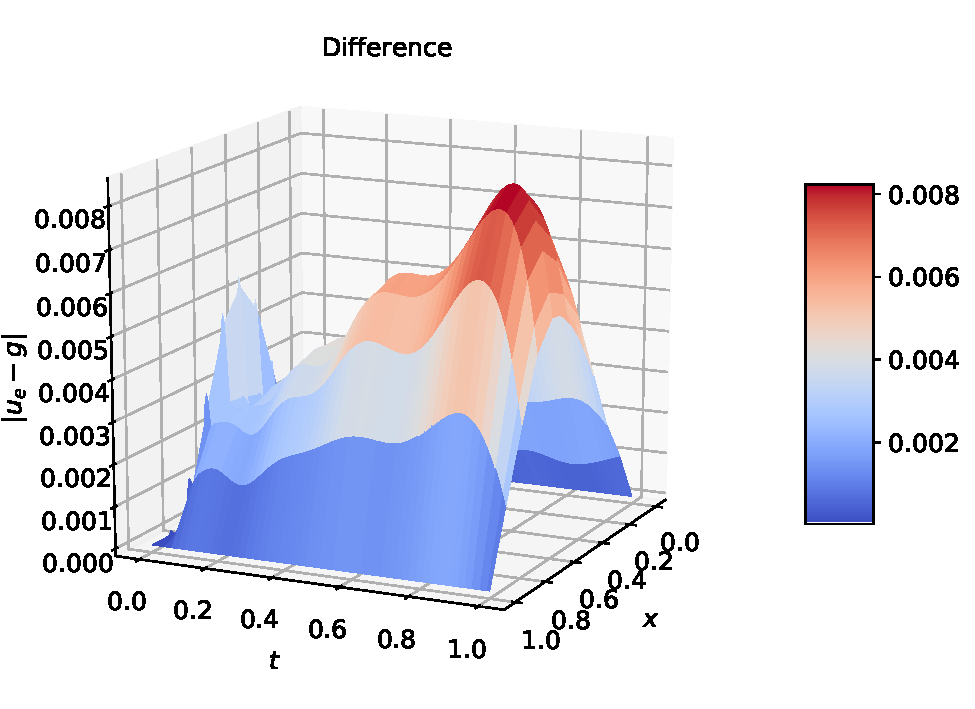
\includegraphics[scale=0.5]{latex/figures/heat_diff_nn1.pdf}}}
\caption{Model 1, Plot solution on the grid FFNN is trained on}
\label{fig:heat_nn1}
\end{figure}

\autoref{fig:heat_nn2} Plot solution on a larger grid than FFNN is trained on, i.e., points must be interpolated

301, 301 points

Max diff: 0.008467176325477247
Mean diff: 0.0032787069037113277

\begin{figure}[H]
\centering
\subfloat[]{{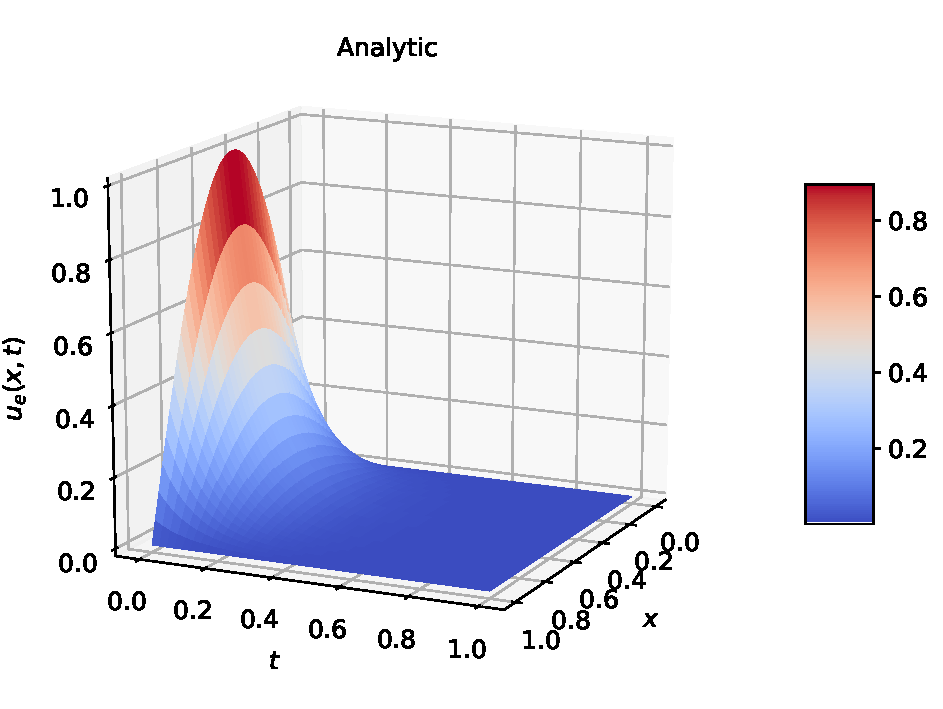
\includegraphics[scale=0.48]{latex/figures/heat_ana_nn2.pdf}}}
\qquad
\subfloat[]{{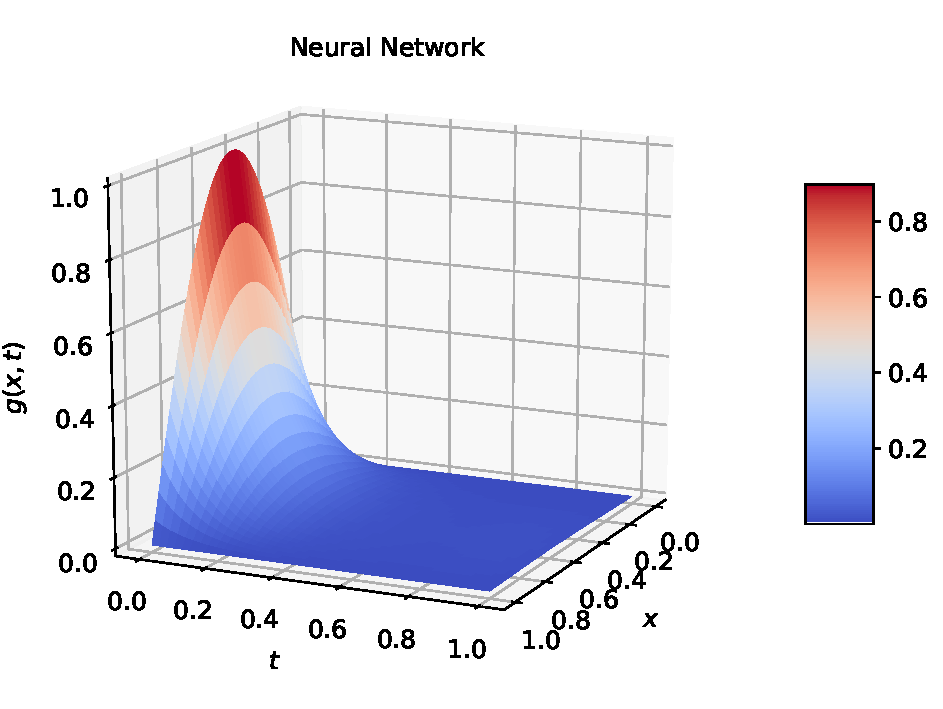
\includegraphics[scale=0.48]{latex/figures/heat_nn2.pdf}}}
\qquad
\subfloat[]{{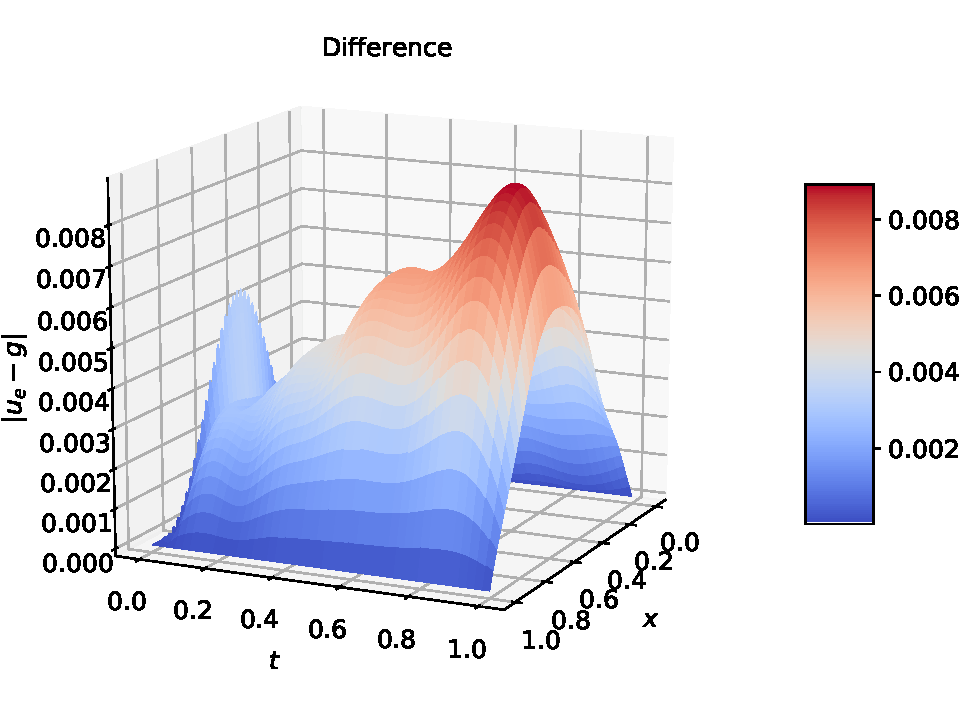
\includegraphics[scale=0.5]{latex/figures/heat_diff_nn2.pdf}}}
\caption{Model 1, Plot solution on a larger grid than FFNN is trained on, i.e., points must be interpolated}
\label{fig:heat_nn2}
\end{figure}

%===============================================================
\subsubsection{FFNN Model 2}
%===============================================================
Model 2: Train on equal number of spatial and temporal points

Nx = 11
Nt = 11
2 layers + output, [150, 50, 1], [tanh, sigmoid, none] 
1000 epochs
Adam, initial lr=0.01
Step: 1000, Loss: 0.008064055285575904
Training FFNN CPU time: 147.62562 secs
Step: 1000, Loss: 0.0027709536906761877
Training FFNN CPU time: 42.11612 secs

\autoref{fig:heat_nn3} Plot solution on the grid FFNN is trained on

Max diff: 0.026960711104318635
Mean diff: 0.0029851059330631173

\begin{figure}[H]
\centering
\subfloat[]{{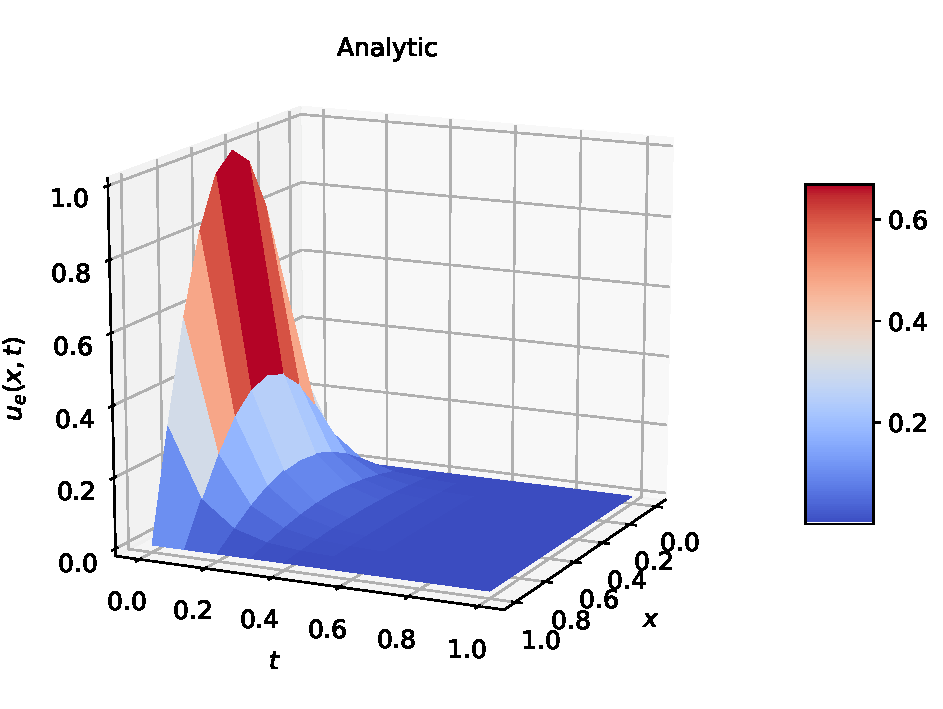
\includegraphics[scale=0.48]{latex/figures/heat_ana_nn3.pdf}}}
\qquad
\subfloat[]{{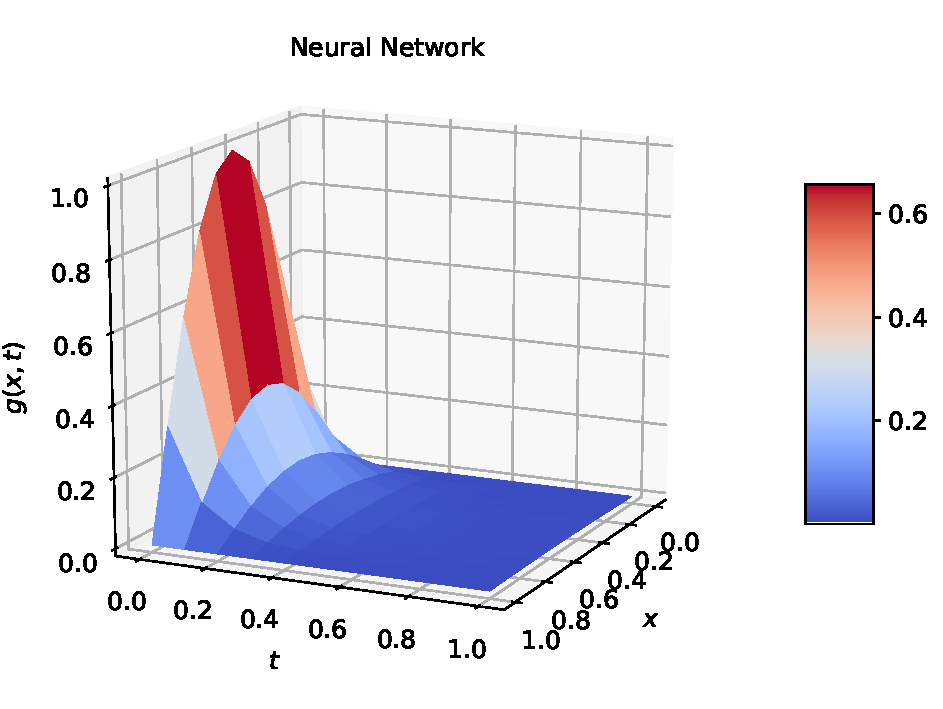
\includegraphics[scale=0.48]{latex/figures/heat_nn3.pdf}}}
\qquad
\subfloat[]{{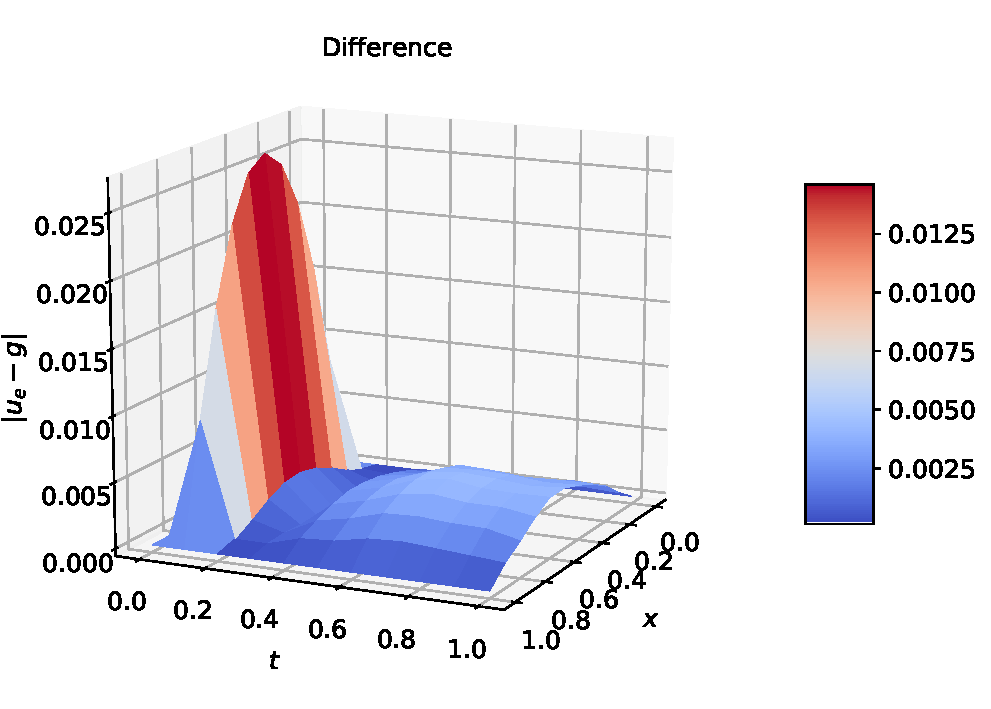
\includegraphics[scale=0.5]{latex/figures/heat_diff_nn3.pdf}}}
\caption{Model 2, Plot solution on the grid FFNN is trained on}
\label{fig:heat_nn3}
\end{figure}

\autoref{fig:heat_nn4} Plot solution on a larger grid than FFNN is trained on, i.e., points must be interpolated

301, 301 points

Max diff: 0.03215260678986426
Mean diff: 0.003950743671390742

\begin{figure}[H]
\centering
\subfloat[]{{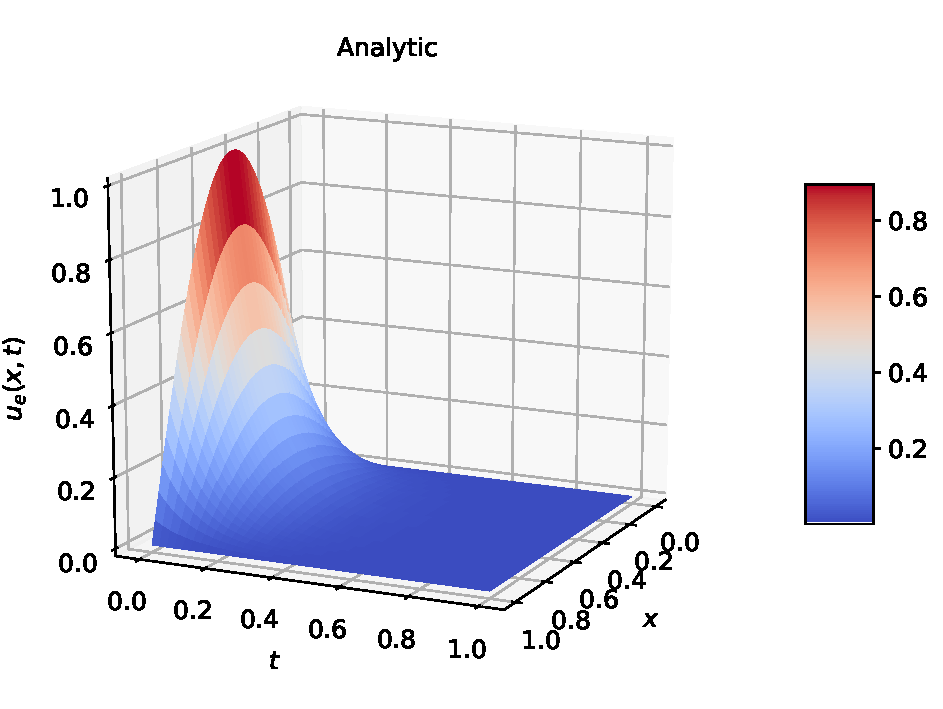
\includegraphics[scale=0.48]{latex/figures/heat_ana_nn4.pdf}}}
\qquad
\subfloat[]{{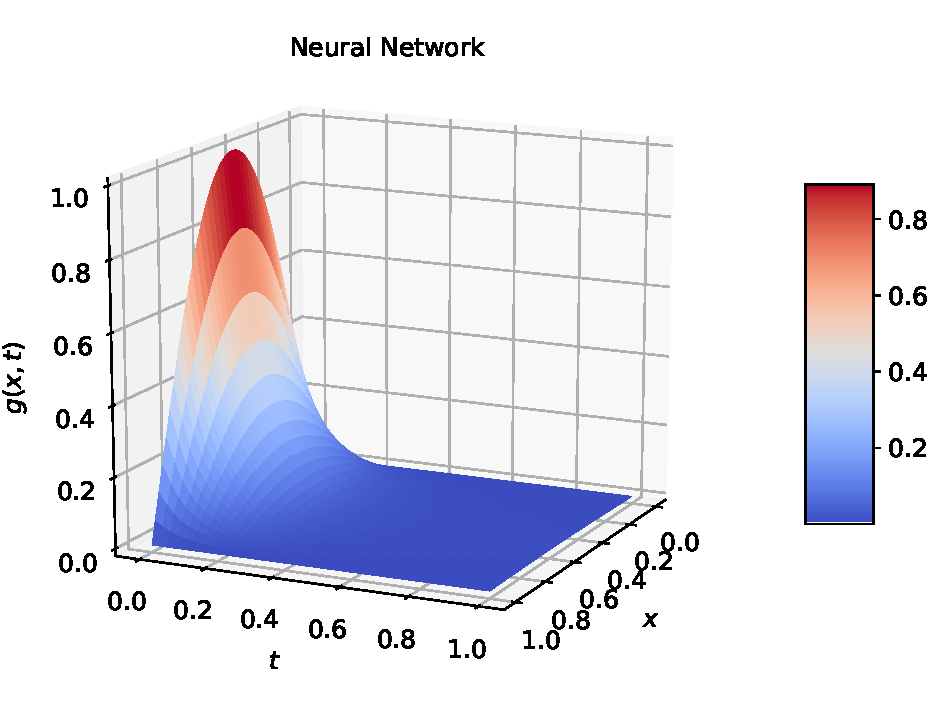
\includegraphics[scale=0.48]{latex/figures/heat_nn4.pdf}}}
\qquad
\subfloat[]{{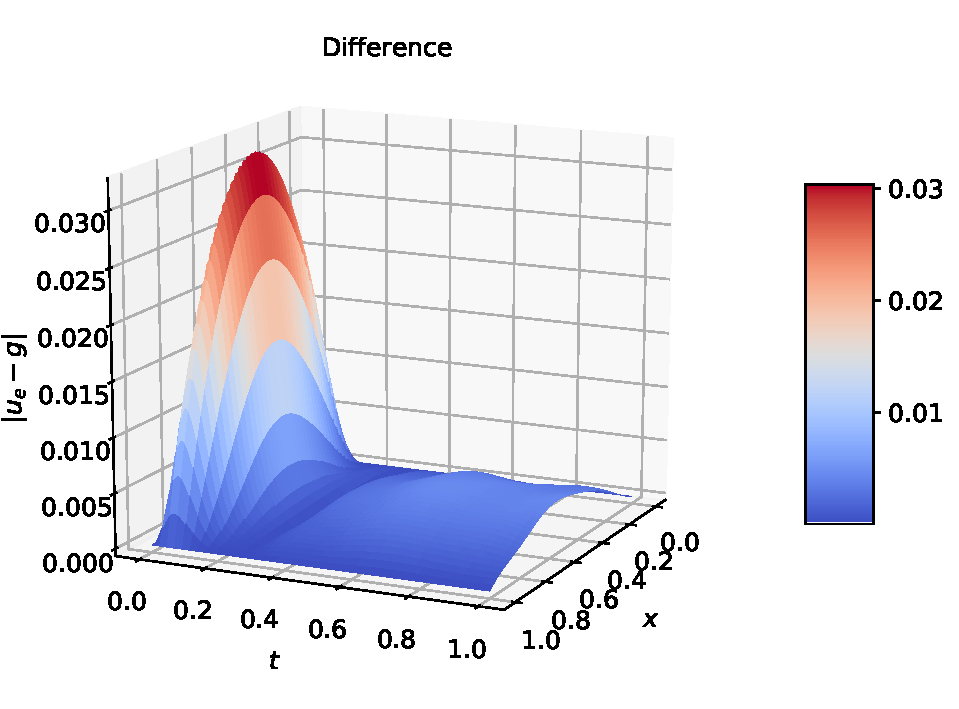
\includegraphics[scale=0.5]{latex/figures/heat_diff_nn4.pdf}}}
\caption{Model 2, Plot solution on a larger grid than FFNN is trained on, i.e., points must be interpolated}
\label{fig:heat_nn4}
\end{figure}


%===============================================================
%===============================================================
\subsection{Eigenvalue Problem}\label{sec:eigenvalue results}
%===============================================================
%===============================================================

Accompanying notebook: \href{https://github.com/nicolossus/FYS-STK4155-Project3/blob/master/notebooks/eigenvalue_tf.ipynb}{eigenvalue\_tf.ipynb}.

%===============================================================
\subsubsection{Benchmark Problem 1}
%===============================================================

\autoref{tab:parabench1} tabulates the problem and model parameters for Benchmark Problem 1 described in \autoref{sec:benchmark problem 1}. 

\begin{table}[H]
\caption{Problem and model parameters for Benchmark Problem 1.}
\centering
\rowcolors{2}{gray!20}{white}
\begin{tabular}{c|c}
\hline
\hline 
Parameter & Numerical Value
\\
\hline 
\hline 
Initial vector & $\bm{x_0}=(1,0,0)$
\\
Simulation time & $T=1$
\\
Number of time points (Euler) & 10\,000
\\
Number of time points (FFNN) & 11
\\
Number of epochs (FFNN) & 2\,000
\\
\hline
\hline 
\end{tabular}
\label{tab:parabench1}
\end{table}


\autoref{fig:benchrun1} shows the results for Benchmark Problem 1. The computed Rayleigh quotients and the absolute error relative to the eigenvalue computed by Numpy are tabulated in \autoref{tab:eigbench1}. 

\begin{figure}[H]
\centering
\subfloat[]{{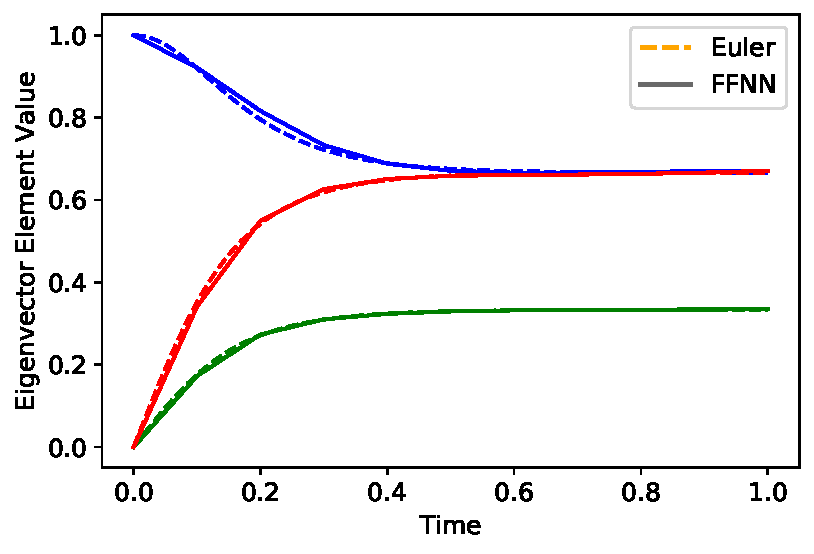
\includegraphics[scale=0.6]{latex/figures/eigvec_comp_benchrun1.pdf}}}
\qquad
\subfloat[]{{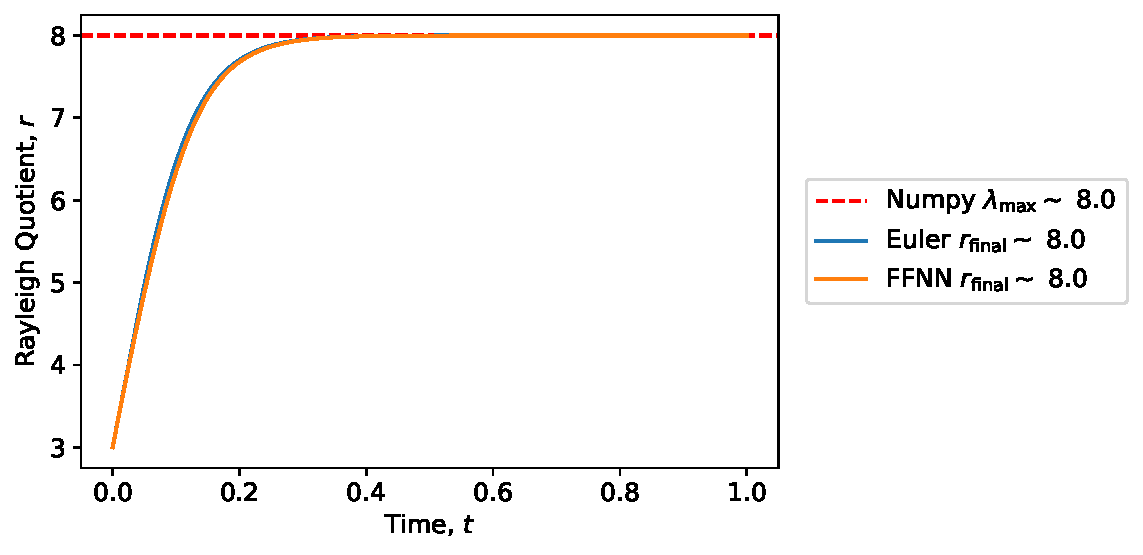
\includegraphics[scale=0.6]{latex/figures/eigval_benchrun1.pdf}}}
\caption{Results for Benchmark Problem 1 with a $3\times 3$ real symmetric matrix $A$. \textbf{(a)} shows the components of the computed steady-state vector as a function of time. The dashed lines are the components computed by Euler's method and the solid lines are computed by the FFNN model. The dotted lines are the normalized eigenvector components corresponding to the largest eigenvalue computed directly from the matrix by Numpy's linalg.eig. \textbf{(b)} shows the computed Rayleigh quotients, $r$, as a function of time for both Euler's method and the FFNN model and the largest eigenvalue, $\lambda_\mathrm{max}$, of the matrix computed by Numpy's inalg.eig as well. The final Rayleigh quotients are rounded to 5 decimal points.}
\label{fig:benchrun1}
\end{figure}

\begin{table}[H]
\caption{The computed Rayleigh quotients at the final simulation time for both Euler's method and the FFNN model. The absolute error relative to the eigenvalue computed by Numpy is also listed.}
\centering
\rowcolors{2}{gray!20}{white}
\begin{tabular}{c|c|c}
\hline
\hline 
Method & Rayleigh Quotient & Absolute Error
\\
\hline 
\hline 
Numpy & 8.0 & –
\\
Euler & 7.99999983 & $1.697 \cdot 10^{-7}$  
\\
FFNN & 7.99999721 & $2.792 \cdot 10^{-6}$
\\
\hline
\hline 
\end{tabular}
\label{tab:eigbench1}
\end{table}

The two solutions shown in \autoref{fig:benchrun1} follow each other closely, and already at $t=1$ they give fairly accurate approximations of the eigenvector corresponding to $\lambda_\mathrm{max}$. The eigenvalue approximation is even more accurate. Euler achieves the highest accuracy and requires far less time to run.

%===============================================================
\subsubsection{Benchmark Problem 2}
%===============================================================

The problem and model parameters for Benchmark Problem 2 are described in \autoref{sec:benchmark problem 2}. In this problem we find the smallest eigenvalue of $A$.

\begin{table}[H]
\caption{Problem and model parameters for Benchmark Problem 2.}
\centering
\rowcolors{2}{gray!20}{white}
\begin{tabular}{c|c}
\hline
\hline 
Parameter & Numerical Value
\\
\hline 
\hline 
Initial vector & $\bm{x_0}=(0.8165, -0.4082,  0.4082)$
\\
Simulation time & $T=3.5$
\\
Number of time points (Euler) & 10\,000
\\
Number of time points (FFNN) & 11
\\
Number of epochs (FFNN) & 2\,000
\\
\hline
\hline 
\end{tabular}
\label{tab:parabench1}
\end{table}

\autoref{fig:benchrun2} shows the results. The computed Rayleigh quotients and the absolute error relative to the eigenvalue computed by Numpy are tabulated in \autoref{tab:eigbench2}. 

\begin{figure}[H]
\centering
\subfloat[]{{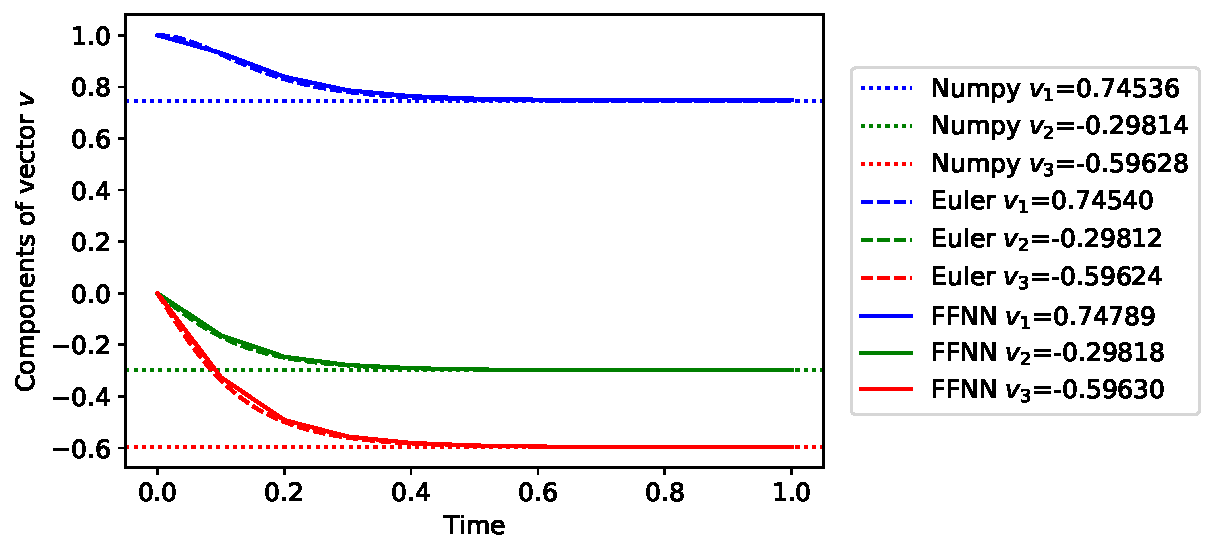
\includegraphics[scale=0.6]{latex/figures/eigvec_comp_benchrun2.pdf}}}
\qquad
\subfloat[]{{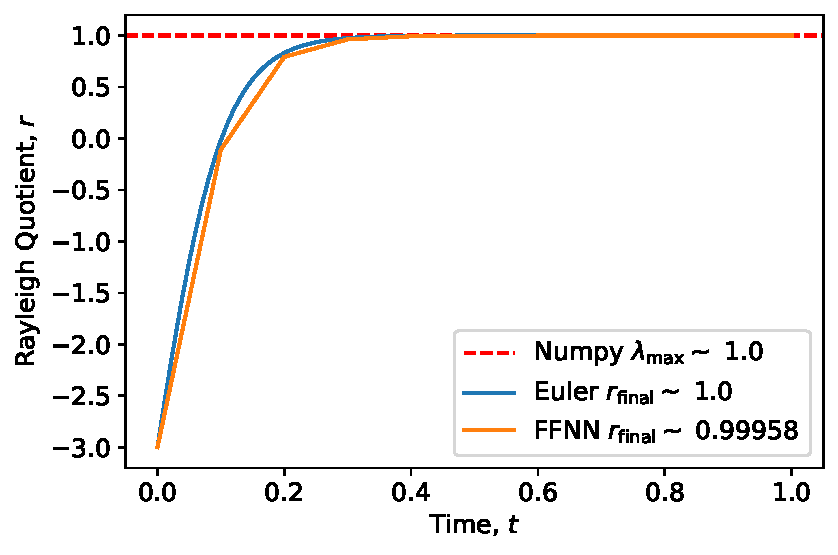
\includegraphics[scale=0.6]{latex/figures/eigval_benchrun2.pdf}}}
\caption{Results for Benchmark Problem 2 with a $3\times 3$ real symmetric matrix $A$. \textbf{(a)} shows the components of the computed steady-state vector as a function of time. The dashed lines are the components computed by Euler's method and the solid lines are computed by the FFNN model. The dotted lines are the normalized eigenvector components corresponding to the largest eigenvalue computed directly from the matrix by Numpy's linalg.eig. \textbf{(b)} shows the computed Rayleigh quotients, $r$, as a function of time for both Euler's method and the FFNN model, and the largest eigenvalue $\lambda_\mathrm{max}$ of the matrix as computed by Numpy's linalg.eig as well. The final Rayleigh quotients are rounded to 5 decimal points.}
\label{fig:benchrun2}
\end{figure}

\begin{table}[H]
\caption{The computed Rayleigh quotients at the final simulation time for both Euler's method and the FFNN model. The absolute error relative to the eigenvalue computed by Numpy is also listed.}
\centering
\rowcolors{2}{gray!20}{white}
\begin{tabular}{c|c|c}
\hline
\hline 
Method & Rayleigh Quotient & Absolute Error
\\
\hline 
\hline 
Numpy & 0.58578644 & –
\\
Euler & 0.58579371 & $7.273 \cdot 10^{-6}$  
\\
FFNN & 0.58579257 & $6.129 \cdot 10^{-6}$
\\
\hline
\hline 
\end{tabular}
\label{tab:eigbench2}
\end{table}

The convergence as $t\to\infty$ was slower this time than in benchmark problem 1, but at $t=3.5$ both the Rayleigh quotients give an eigenvalue approximation that is accurate to five decimal places.

%===============================================================
\subsubsection{Benchmark Problem 3}
%===============================================================

\autoref{tab:parabench3} tabulates the problem and model parameters for Benchmark Problem 3 described in \autoref{sec:benchmark problem 3}. 

\begin{table}[H]
\caption{Problem and model parameters for Benchmark Problem 3.}
\centering
\rowcolors{2}{gray!20}{white}
\begin{tabular}{c|c}
\hline
\hline 
Parameter & Numerical Value
\\
\hline 
\hline 
Initial vector & $\bm{x_0}=(-0.707, 0.707, 0)$
\\
Simulation time & T=1
\\
Number of time points (Euler) & 10\,000
\\
Number of time points (FFNN) & 11
\\
Number of epochs (FFNN) & 2000
\\
\hline
\hline 
\end{tabular}
\label{tab:parabench3}
\end{table}


\autoref{fig:benchrun3} shows the results for Benchmark Problem 3. The computed Rayleigh quotients and the absolute error relative to the eigenvalue computed by Numpy are tabulated in \autoref{tab:eigbench3}.

\begin{figure}[H]
\centering
\subfloat[]{{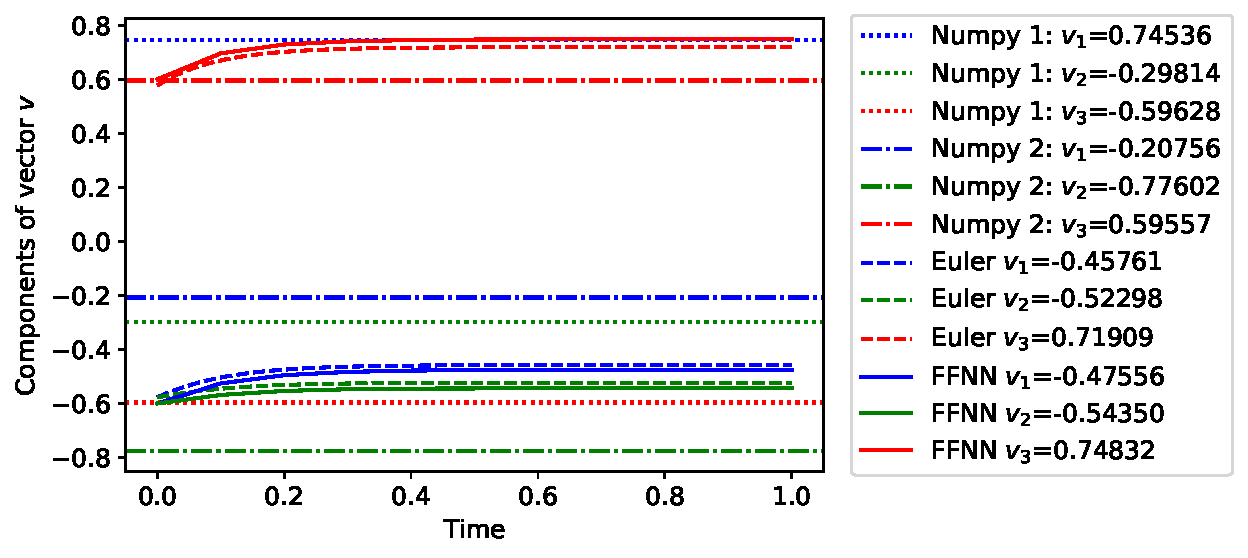
\includegraphics[scale=0.6]{latex/figures/eigvec_comp_benchrun3.pdf}}}
\qquad
\subfloat[]{{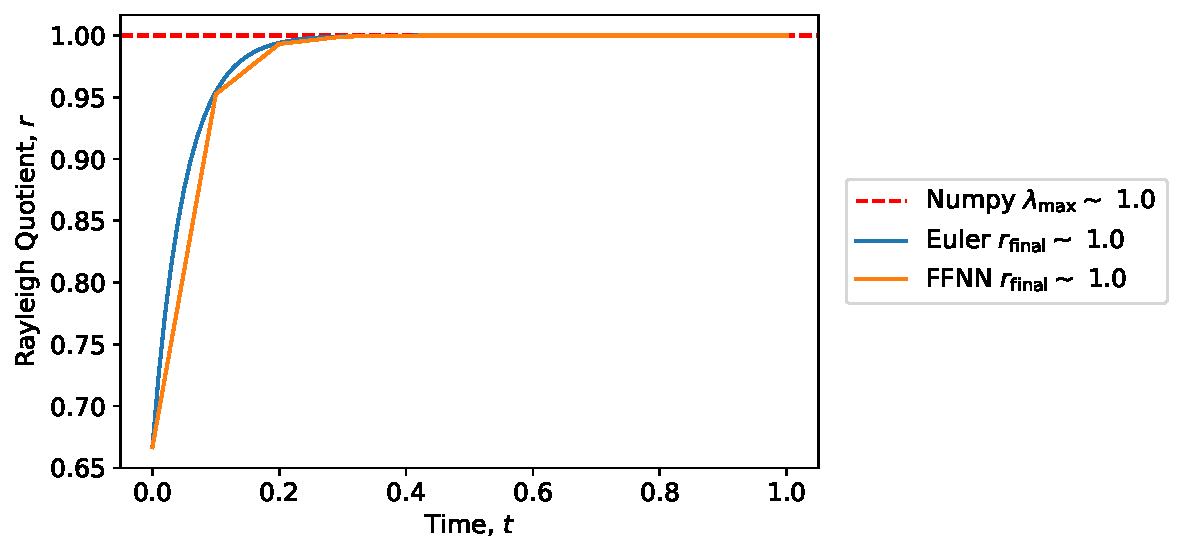
\includegraphics[scale=0.6]{latex/figures/eigval_benchrun3.pdf}}}
\caption{Results for Benchmark Problem 2 with a $3\times 3$ real symmetric matrix $-A$. \textbf{(a)} shows the components of the computed steady-state vector as a function of time. The dashed lines are the components computed by Euler's method and the solid lines are computed by the FFNN model. The dotted lines are the normalized components of the eigenvector corresponding to the smallest eigenvalue, as computed by Numpy's linalg.eig. All lines corresponding to the same vector component are here on top of each other. \textbf{(b)} shows the computed Rayleigh quotients, $r$, as a function of time for both Euler's method and the FFNN model. Both the largest and the smallest eigenvalue as calculated by linalg.eig are also shown. Three of the four lines are all at the same spot in the bottom. The numbers are rounded to 5 decimal points.}
\label{fig:benchrun3}
\end{figure}

\begin{table}[H]
\caption{The computed Rayleigh quotients at the final simulation time for both Euler's method and the FFNN model. The absolute error relative to the eigenvalue computed by Numpy is also listed.}
\centering
\rowcolors{2}{gray!20}{white}
\begin{tabular}{c|c|c}
\hline
\hline 
Method & Rayleigh Quotient & Absolute Error
\\
\hline 
\hline 
Numpy & 2.0 & –
\\
Euler & 2.0 & $3.553 \cdot 10^{-15}$  
\\
FFNN & 2.0 & $3.526 \cdot 10^{-12}$
\\
\hline
\hline 
\end{tabular}
\label{tab:eigbench3}
\end{table}

As mentioned in \autoref{sec:benchmark problem 3}, the starting vector $\bm{x_0}$ is itself an eigenvector of $A$, so the point of convergence is just $\bm{x_0}$ itself. Both methods did well in approximating the constant function. This is particularly easy for the Euler method, which as usual came out on top.

%===============================================================
\subsubsection{Benchmark Problem 4}
%===============================================================

\autoref{tab:parabench4} tabulates the problem and model parameters for Benchmark Problem 4 described in \autoref{sec:benchmark problem 4}. 

\begin{table}[H]
\caption{Problem and model parameters for Benchmark Problem 4.}
\centering
\rowcolors{2}{gray!20}{white}
\begin{tabular}{c|c}
\hline
\hline 
Parameter & Numerical Value
\\
\hline 
\hline 
Initial vector & $\bm{x_0}=(0.208, 0.347, 0.365, 0.123, 0.648, 0.518)$
\\
Simulation time & $T=10$
\\
Number of time points (Euler) & 51, 101, 501, 1001
\\
Number of time points (FFNN) & 5, 11, 51, 101
\\
Number of epochs (FFNN) & $2\,000$
\\
\hline
\hline 
\end{tabular}
\label{tab:parabench4}
\end{table}

\begin{figure}[H]
\centering
\subfloat[]{{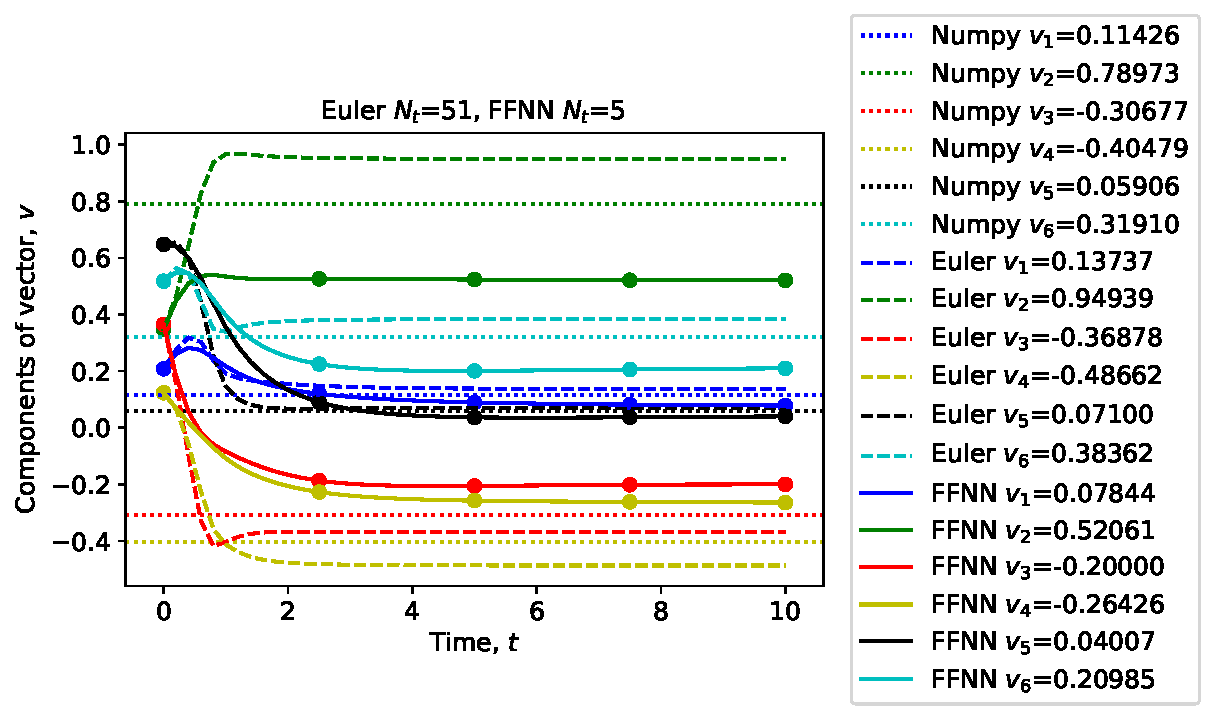
\includegraphics[scale=0.7]{latex/figures/eigvec_comp_run66a.pdf}}}
\qquad
\subfloat[]{{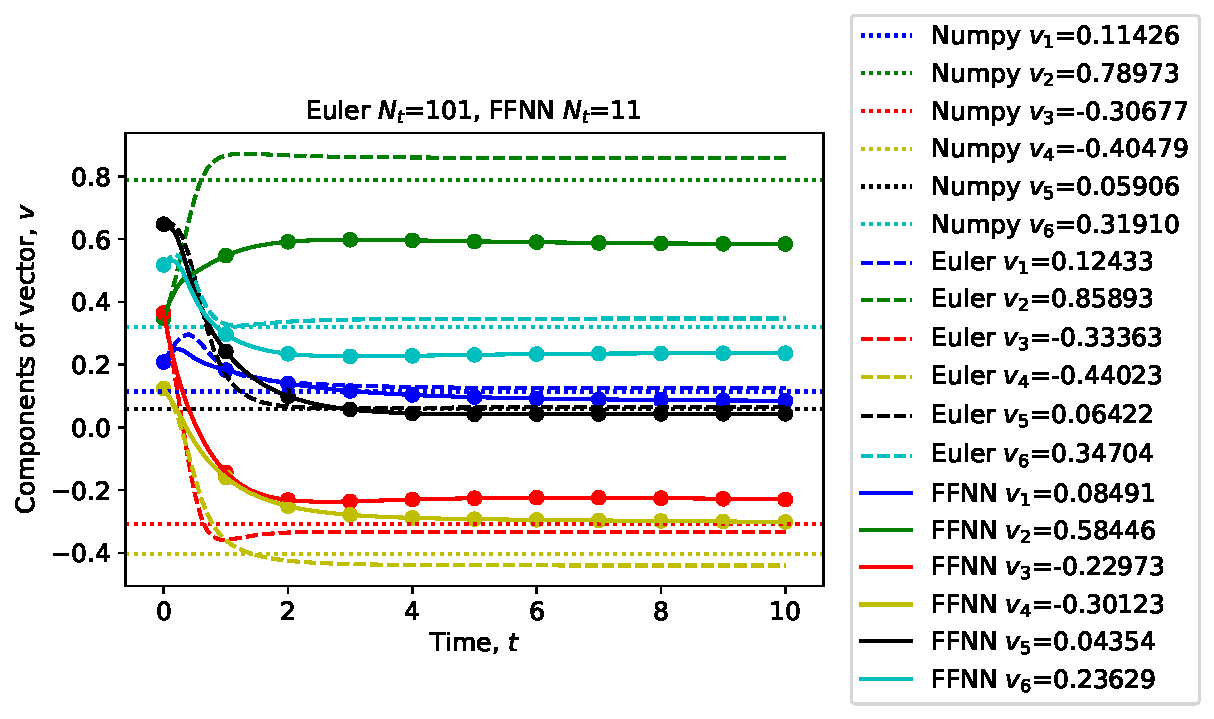
\includegraphics[scale=0.7]{latex/figures/eigvec_comp_run66b.pdf}}}
\caption{Results for Benchmark Problem 4 with a $6\times 6$ real symmetric matrix $A$. The figure shows the time evolution of the vector components of the solution computed by Euler's method and the FFNN solution with, respectively, the following time steps: \textbf{(a)} 51 and 5, \textbf{(b)} 101 and 11. The points where we have trained the FFNN are marked with dots on the graphs.}
\label{fig:benchrun4_comp_1}
\end{figure}

\begin{figure}[H]
\centering
\subfloat[]{{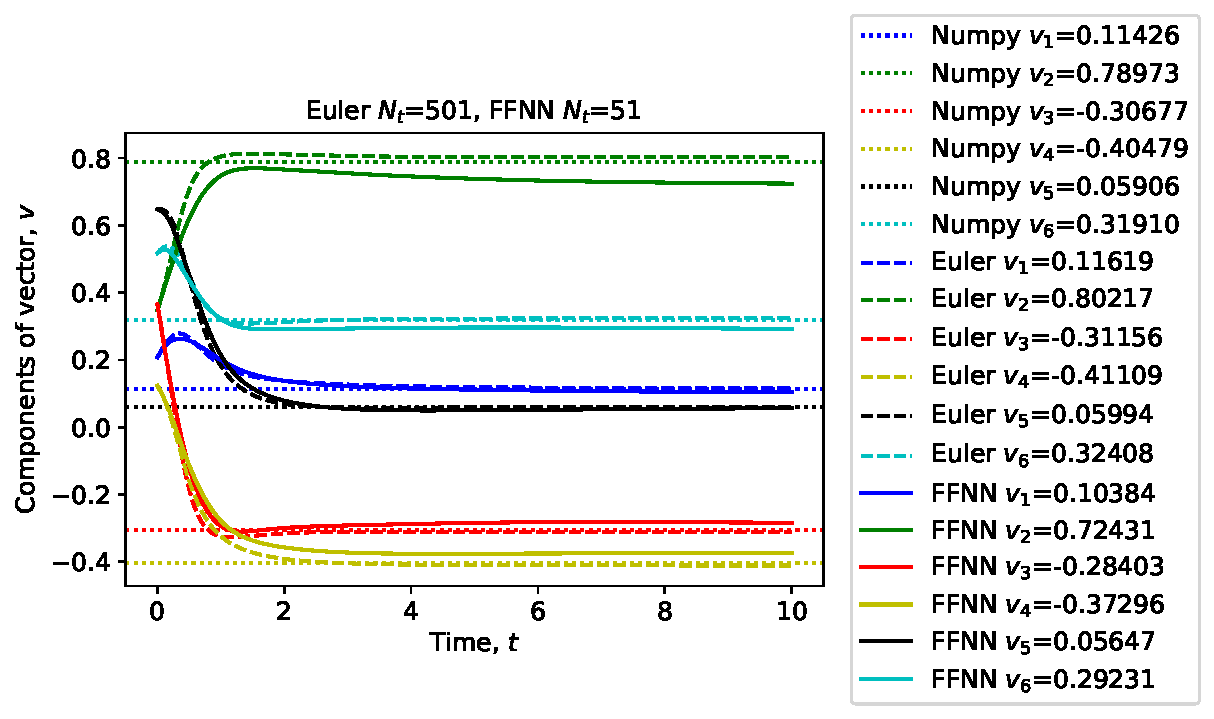
\includegraphics[scale=0.7]{latex/figures/eigvec_comp_run66c.pdf}}}
\qquad
\subfloat[]{{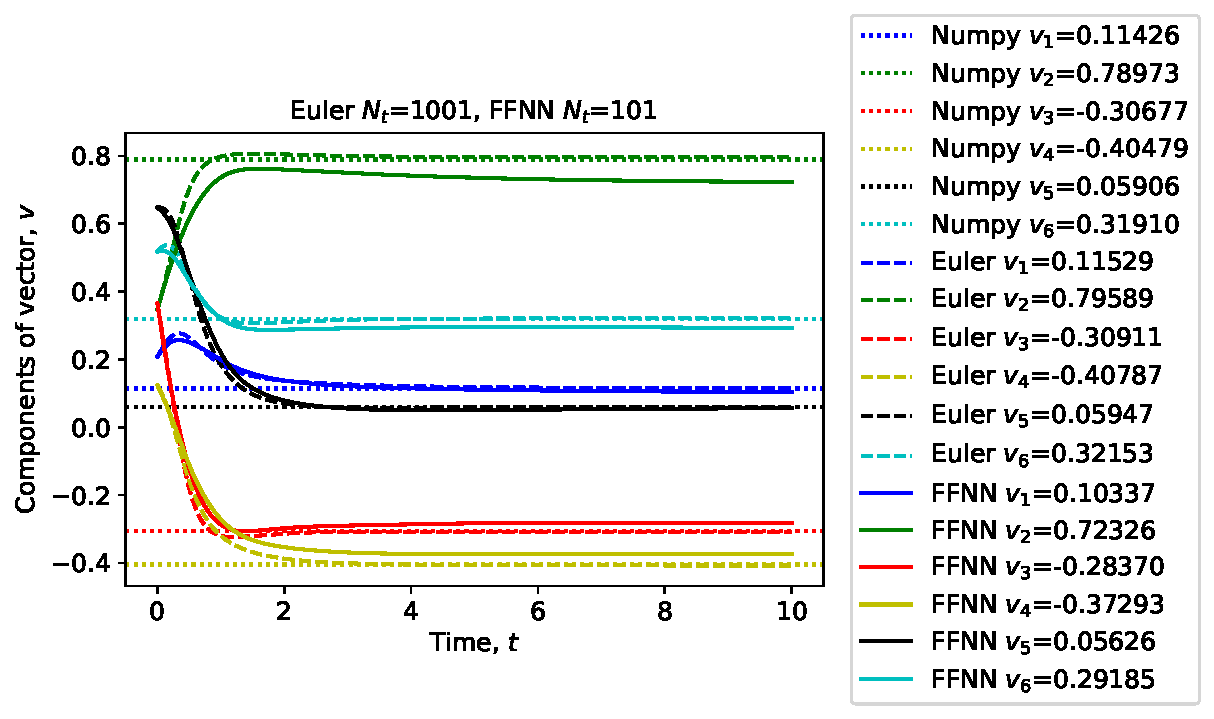
\includegraphics[scale=0.7]{latex/figures/eigvec_comp_run66d.pdf}}}
\caption{Results for Benchmark Problem 4 with a $6\times 6$ real symmetric matrix $A$. The figure shows the time evolution of the vector components of the solution computed by Euler's method and the FFNN solution with, respectively, the following time steps: \textbf{(a)} 501 and 51, \textbf{(b)} 1001 and 101.}
\label{fig:benchrun4_comp_2}
\end{figure}

\begin{figure}[H]
\centering
\subfloat[]{{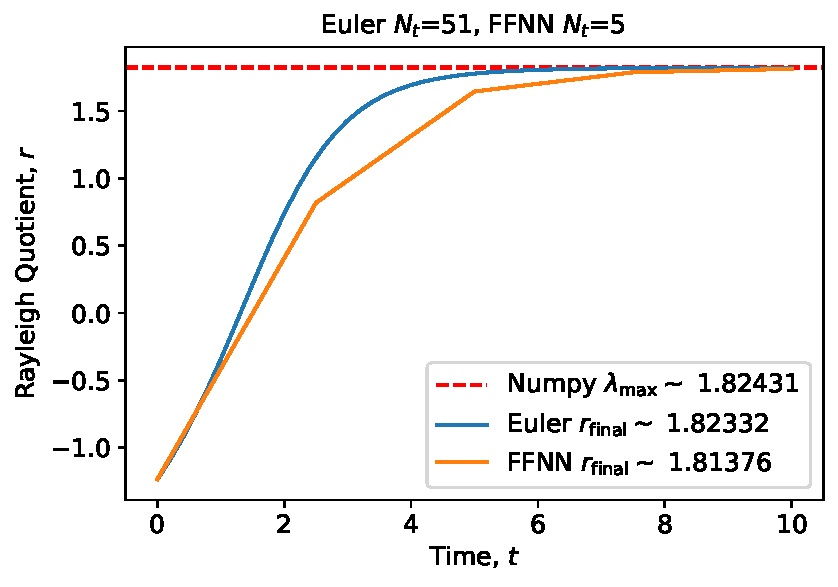
\includegraphics[scale=0.5]{latex/figures/eigval_run66a.pdf}}}
\qquad
\subfloat[]{{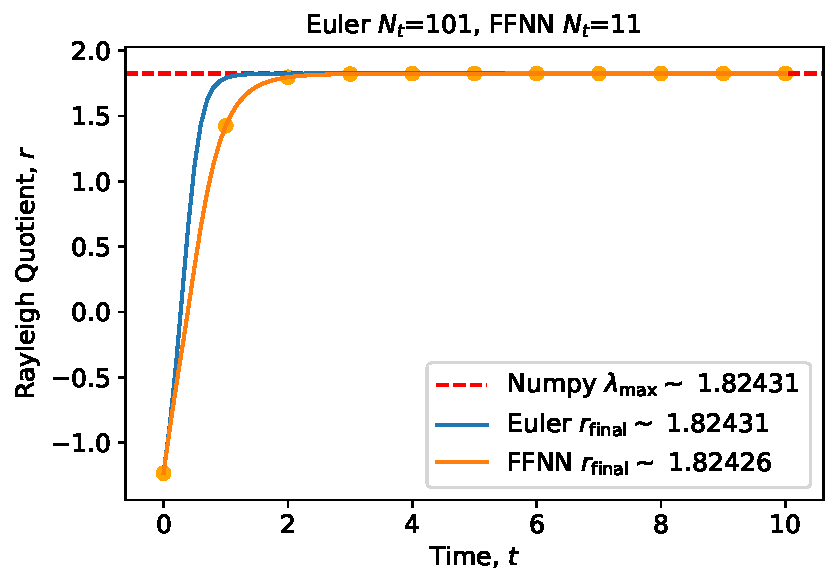
\includegraphics[scale=0.5]{latex/figures/eigval_run66b.pdf}}}
\qquad
\subfloat[]{{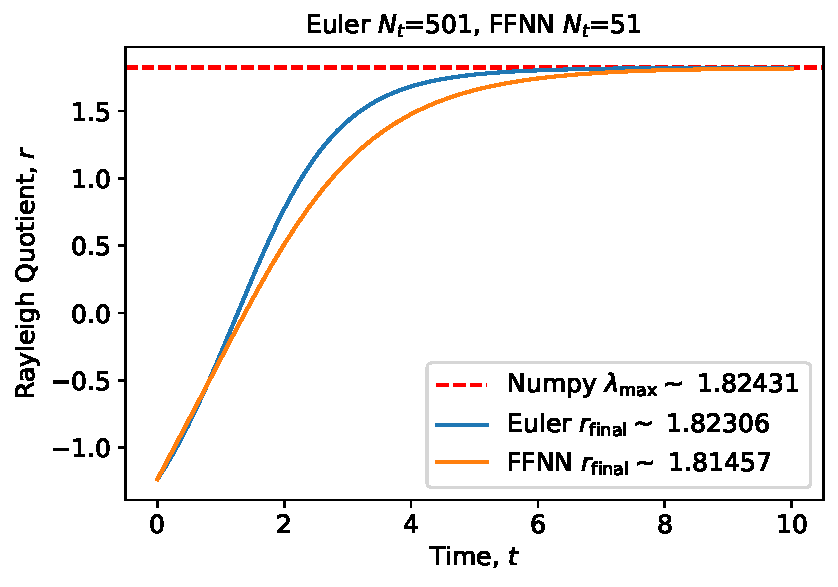
\includegraphics[scale=0.5]{latex/figures/eigval_run66c.pdf}}}
\qquad
\subfloat[]{{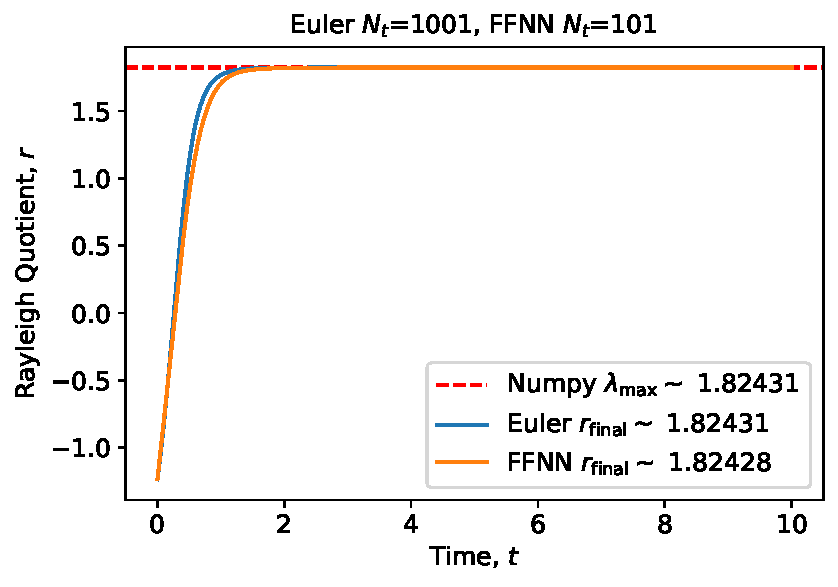
\includegraphics[scale=0.5]{latex/figures/eigval_run66d.pdf}}}
\caption{Results for Benchmark Problem 5 with a $6\times 6$ real symmetric matrix, $A$. The figure shows the time evolution of the Rayleigh quotient computed by Euler's method and the FFNN model with, respectively, the following time steps: \textbf{(a)} 51 and 5, \textbf{(b)} 101 and 11, \textbf{(c)} 501 and 51, \textbf{(d)} 1001 and 101. For number of time steps equal to 5 and 11, the points where we have trained the FFNN are marked with dots on the graph.}
\label{fig:benchrun4}
\end{figure}

The final Rayleigh quotients computed at different time steps and the absolute error relative to the eigenvalue computed by Numpy are tabulated in \autoref{tab:eigbench4}.

\begin{table}[H]
\caption{The computed Rayleigh quotients at the final simulation time for both Euler's method and the FFNN model with different time steps. The absolute error relative to the eigenvalue computed by Numpy is also listed.}
\centering
\rowcolors{2}{gray!20}{white}
\begin{tabular}{c|c|c|c}
\hline
\hline 
Method & Number of Time Steps & Rayleigh Quotient & Absolute Error
\\
\hline 
\hline 
Euler & 51 & 1.82431291 & $4.781\cdot10^{-11}$
\\
Euler & 101 & 1.82431291 & $2.060\cdot10^{-9}$
\\
Euler & 501 & 1.82431290 & $1.505\cdot10^{-8}$
\\
Euler & 1001 & 1.82431289 & $1.847 \cdot10^{-8}$
\\
FFNN & 5 & 1.82423239 & $8.052\cdot10^{-5}$
\\
FFNN & 11 & 1.82425943 & $5.348\cdot10^{-5}$
\\
FFNN & 51 & 1.82428079 & $3.212\cdot10^{-5}$
\\
FFNN & 101 & 1.82427677 & $3.615\cdot10^{-5}$
\\
\hline
\hline 
\end{tabular}
\label{tab:eigbench4}
\end{table}

For a small number of time steps neither method achieves a good accuracy in approximating the eigenvector. The eigenvalue approximation, however, is not as sensitive for the number of time steps, and does not vary at the same rate.

At least for dense time points, the accuracy of the FFNN can be improved by increasing the number of epochs, but of course at the cost of increased computational requirements.

The eigenvalue approximation actually, and perhaps interestingly, got worse with smaller time steps for the Euler method, even though the eigenvalue approximation clearly improved. For the FFNN solution we saw improvements for both the eigenvector and the eigenvalue until the number of time points reached 51. At 101 time points, the accuracy fell slightly.

An advantage with the FFNN solution over the one from the Euler method is that we get a function that is smooth, i.e. infinitely differentiable, in every point, not a piecewise linear one.

